%Version 3.1 December 2024 -- Springer Nature LaTeX template (sn-jnl), official package
%downloaded from resource-cms.springernature.com on 2026-10-23 (see report/final/README.md).
%Numbered Math and Physical Sciences reference style.
\documentclass[pdflatex,sn-mathphys-num]{sn-jnl}

\usepackage{graphicx}%
\usepackage{multirow}%
\usepackage{amsmath,amssymb,amsfonts}%
\usepackage{amsthm}%
\usepackage{mathrsfs}%
\usepackage[title]{appendix}%
\usepackage{xcolor}%
\usepackage{textcomp}%
\usepackage{manyfoot}%
\usepackage{booktabs}%
\usepackage{array}%
\usepackage{tabularx}%
\usepackage{xurl}%
\usepackage{tikz}%
\usetikzlibrary{arrows.meta,positioning,fit,calc,backgrounds}%

\theoremstyle{thmstyleone}%
\newtheorem{theorem}{Theorem}%

\raggedbottom
\emergencystretch=3em
\sloppy

% Values filled in from the last audit runs (see report/final/evidence_ledger.md).
\newcommand{\CISLRRESULT}{answering from all 262 words on the 609 clips, top-1 was 9.6\% (seeds 9.5, 8.7, 10.5; top-5 22.4\%), and on the 98 CISLR clips of deployed words with the 50-word restriction it was 29.3\% (29.6, 27.6, 30.6; chance 2\%), against 85.9\% on INCLUDE. The landmark model therefore transfers far better than the earlier pixel-only checkpoints, but most of its INCLUDE accuracy does not carry over to another corpus. iSign and CISLR come from the same research group, and we did not check whether any of the unlabelled iSign pretraining videos also appear in CISLR}
\newcommand{\SRAPPRESULT}{50 clips copied at 180p, JPEG 40: bicubic 32, SR-L1 39, SR-GAN v2 37 correct; in each arm 50 of 50 outcomes match the study's seed-0 result file}
\newcommand{\LATMS}{20.9\,ms}
\newcommand{\LATIQR}{20.2--21.9\,ms}

% ---------------------------------------------------------------------------
% Evidence links. Every code and result link is pinned to the audited commit.
% \ev{path#anchor}{shown text}: the shown text is typeset as a breakable URL.
% ---------------------------------------------------------------------------
\newcommand{\repo}{https://github.com/not-good-keeper/compact-vit-sign-language/blob/ea092f3e25124fcd8929929900e53879d7084943}
\newcommand{\treeurl}{https://github.com/not-good-keeper/compact-vit-sign-language/tree/ea092f3e25124fcd8929929900e53879d7084943}
\newcommand{\ev}[2]{\href{\repo/#1}{\nolinkurl{#2}}}
\newcommand{\evdir}[2]{\href{\treeurl/#1}{\nolinkurl{#2}}}
\newcommand{\new}[1]{\nolinkurl{#1}}
\newenvironment{evidence}{\par\smallskip\noindent\begin{minipage}{\linewidth}\footnotesize\raggedright\setlength{\parskip}{2pt}}{\end{minipage}\par\smallskip}
\newcommand{\evitem}[1]{\par\textbf{#1}\enspace}
\newcolumntype{L}[1]{>{\raggedright\arraybackslash\hspace{0pt}}p{#1}}
\newcolumntype{Y}{>{\raggedright\arraybackslash\hspace{0pt}}X}

\definecolor{cA}{HTML}{2a78d6}
\definecolor{cB}{HTML}{eb6834}
\definecolor{cC}{HTML}{1baf7a}
\definecolor{cD}{HTML}{eda100}
\definecolor{ink2}{HTML}{52514e}
\definecolor{panel}{HTML}{f3f2ef}
\tikzset{
  box/.style={draw=ink2, rounded corners=2pt, align=center, font=\footnotesize, inner sep=3pt, minimum height=7mm, fill=white},
  stage/.style={box, fill=panel},
  arr/.style={-{Stealth[length=2.2mm]}, draw=ink2, line width=0.6pt},
  lab/.style={font=\scriptsize, text=ink2, align=center},
}

\begin{document}

\title[Compact factorised ViT for isolated ISL words]{ISL-ViT-Tiny: A Compact Factorised Vision Transformer for Isolated-Word Indian Sign Language Recognition, Evaluated on Held-Out Recording Sessions}

\author[1]{\fnm{Yalamanchi} \sur{Kushal}}
\author[1]{\fnm{Nethi} \sur{Kushala Kumar}}
\author[1]{\fnm{Dhruseek} \sur{Rishi Menon}}

\affil[1]{\orgname{Amrita School of Computing, Amrita Vishwa Vidyapeetham}, \orgaddress{\city{Coimbatore}, \country{India}}}

\abstract{Word-level recognition of Indian Sign Language (ISL) on a wearable device has two constraints that published ISL work rarely reports together: the model must be small, and the accuracy figure must come from recording conditions the model has not seen. We built ISL-ViT-Tiny, a factorised spatio-temporal Vision Transformer that reads three detected crops per frame (left hand, right hand, face) over 16 frames, adds 21 hand-joint landmarks per hand to the hand tokens, and is trained on INCLUDE (262 words) after masked-image pretraining on iSign. We evaluated it on INCLUDE recording sessions held out as whole blocks of camera capture identifiers, a proxy for session independence rather than a signer-independent test. On the 472 held-out clips of the 50 deployed words, with predictions restricted to those words and six-view test-time augmentation, the released 4-bit model (2,069,700 bytes; 3,894,214 parameters) reached 85.9\% mean top-1 accuracy over three seeds (96.4\% top-5); answering from all 262 words gave 72.0\%. Landmarks added 12.8 points over a pixel-only control trained with the same recipe, and quantisation-aware training recovered most of the 3.1 points that post-training 4-bit rounding lost. One recipe scored 98.5\% on a random-video split and 70.1\% on held-out sessions. A learned super-resolution front end raised 180p accuracy from 61.0\% to about 75.5\%, but the adversarial loss gave a reliable gain in only 2 of 9 controlled comparisons. On a second corpus, CISLR, the released model reached only 29.3\% on the deployed words, and it has not been validated on new signers or on wearable hardware.}

\keywords{Indian Sign Language recognition, Vision Transformer, spatio-temporal modelling, hand landmarks, 4-bit quantisation, evaluation protocol, super-resolution GAN}

\maketitle

% ===========================================================================
\section{Introduction}\label{sec:intro}
% ===========================================================================

Indian Sign Language is the primary language of a large Deaf community in India; the INCLUDE authors cite more than five million users~\cite{sridhar2020include}. An automatic recogniser for isolated ISL words could support communication with non-signers, and a camera on a pair of smart glasses is one place such a recogniser could run. That target sets two requirements that pull against each other. The network must fit a memory and compute budget far below that of standard video models, and its reported accuracy must describe what happens when the signer, room and lighting differ from the training recordings.

The second requirement is the harder one to meet with public ISL data. INCLUDE, the main labelled word-level corpus, contains 4,287 videos of 263 words recorded by experienced signers~\cite{sridhar2020include}; the copy used here has 4,257 usable clips of 262 words. A word has a median of 15 clips, many of them back-to-back takes of the same signer in the same session. A random split of such data puts near-identical takes on both sides of the train/test boundary, so a high score can reflect recognition of the recording rather than of the sign. The problem is not specific to sign language: Kapoor and Narayanan document train--test leakage across machine-learning-based science~\cite{kapoor2023leakage}. Within sign language, AUTSL reports 95.95\% for its baselines on random splits and 62.02\% on its user-independent split~\cite{sincan2020autsl}. Published INCLUDE results of 85.6\% (263 words) and 94.5\% (INCLUDE-50)~\cite{sridhar2020include}, and 93.5 to 94.7\% for pose-based models~\cite{selvaraj2022openhands}, were obtained on the dataset's own split; Section~\ref{sec:res:protocol} shows how much such splits can inflate accuracy on this corpus.

Transformer video models~\cite{arnab2021vivit,bertasius2021timesformer} and pose-based sign recognisers~\cite{bohacek2022spoter,jiang2021samslr,selvaraj2022openhands} give strong results on sign data, and recent work targets edge hardware~\cite{lamaakal2026tinymslr,venkatappa2026kannada}. In the sources we reviewed (Section~\ref{sec:related}) we did not find an ISL word recogniser that reports, in one place, a hard size budget, a measured quantisation cost, a split that holds out whole recording sessions, and an application tested against the offline evaluation.

The project's objectives were to (i) reach at least 75\% top-1 accuracy on 50 deployable words measured on held-out recording sessions; (ii) keep the model near 2\,MB; (iii) use an evaluation protocol that does not reward memorising a session; (iv) integrate the model into a working interface; and (v) test a generative adversarial network (GAN) in a position where its contribution can be isolated. This report audits the implementation at commit \texttt{ea092f3} of the public repository and documents what was built and measured.

The contributions, stated at the level the evidence supports, are:
\begin{enumerate}
\item A task-specific compact recogniser: a factorised spatial-then-temporal Transformer over hand and face crops, with crop position, detection status and normalised hand-joint features added to the crop tokens (Section~\ref{sec:method:model}). The components are established; the combination and its sizing to a 2\,MB budget are ours.
\item Controlled measurements on one fixed test set: the landmark stream (+12.8 points, paired $p\le 5\times10^{-9}$ in each seed), post-training versus quantisation-aware 4-bit compression, temporal length, crop resolution and training duration (Section~\ref{sec:results}).
\item A recording-session-aware evaluation built from capture identifiers, with a matched measurement of how much a random split inflates accuracy (about 28 points for one recipe), and a statement of what the proxy does not establish (Sections~\ref{sec:method:eval} and~\ref{sec:limits}).
\item An integrated application whose prediction route reproduced the offline per-clip outcome for three classifier variants and three low-resolution front ends, on 50 held-out clips each (Section~\ref{sec:res:app}).
\item A controlled super-resolution study that separates the benefit of a learned upscaler from the benefit of the adversarial loss (Section~\ref{sec:res:gan}).
\end{enumerate}

% ===========================================================================
\section{Related work}\label{sec:related}
% ===========================================================================

\paragraph{ISL datasets and recognisers.} INCLUDE~\cite{sridhar2020include} is the reference labelled corpus for isolated ISL words; its best model, a pretrained feature extractor and encoder with a trained decoder, reached 85.6\% on 263 words and 94.5\% on the 50-word subset. CISLR~\cite{joshi2022cislr} has a vocabulary of about 4,700 words with roughly 1.5 videos per word, so its authors frame recognition as a one-shot task; their prototype baseline reached 16.81\% top-1 on CISLR v1.0-a. iSign~\cite{joshi2024isign} provides a large collection of ISL video--sentence pairs and benchmark tasks. Recent ISL systems include a CNN--ViT conversational agent reporting 97.5\% accuracy under optimised conditions on a domain-specific dataset~\cite{nedungadi2025vit} and a two-handed dynamic ISL recogniser~\cite{govindharajalu2025isl}; Damdoo and Kumar survey the field~\cite{damdoo2025survey}.

\paragraph{Video and pose models for sign recognition.} The Vision Transformer~\cite{dosovitskiy2021vit} and the data-efficient DeiT training recipe~\cite{touvron2021deit} made patch-token models practical on modest datasets. For video, ViViT~\cite{arnab2021vivit} studies variants that factorise spatial and temporal attention, and TimeSformer~\cite{bertasius2021timesformer} compares divided space--time attention with joint attention. Sign Language Transformers~\cite{camgoz2020slt} applied Transformers to continuous recognition and translation. Pose-based recognisers operate on body and hand keypoints: SPOTER~\cite{bohacek2022spoter} normalises hand poses in a local coordinate frame and reports 63.18\% on WLASL100; SAM-SLR~\cite{jiang2021samslr} fuses skeleton, RGB and depth streams; SignBERT~\cite{hu2021signbert} pretrains a hand-model-aware representation; OpenHands~\cite{selvaraj2022openhands} releases pose-based models for six sign languages and reports 93.5\% (SL-GCN) on INCLUDE, rising to 94.7\% with self-supervised pretraining. Our model combines the two families: pixels of detected regions, plus hand landmarks from MediaPipe~\cite{lugaresi2019mediapipe,zhang2020mphands} added to the visual tokens rather than processed by a separate graph network.

\paragraph{Compact models and quantisation.} Integer quantisation with simulated rounding during training~\cite{jacob2018quant} and the straight-through gradient estimator~\cite{bengio2013ste} are the standard basis of quantisation-aware training; Nagel et al. review post-training and quantisation-aware methods~\cite{nagel2021whitepaper}. Group-wise scales, which give each block of weights its own scale, appear in Q-BERT~\cite{shen2020qbert} and GPTQ~\cite{frantar2023gptq}. For sign recognition at the edge, TinyMSLR~\cite{lamaakal2026tinymslr} reports fewer than 2.7\,M parameters and 7.2\,MB on a 20-class isolated-sign benchmark built from two corpora with a signer-independent protocol, and a Kannada Sign Language study~\cite{venkatappa2026kannada} deploys quantised LSTM and Transformer models on a smartphone while noting that its split was not signer-independent.

\paragraph{Evaluation protocols.} WLASL~\cite{li2020wlasl} collects more than 2,000 words from over 100 signers, and AUTSL~\cite{sincan2020autsl} publishes a user-independent benchmark split and reports the random-versus-user-independent gap quoted in Section~\ref{sec:intro}. INCLUDE ships without signer identifiers, so a signer-disjoint split cannot be built from its metadata; the protocol in Section~\ref{sec:method:eval} reconstructs recording sessions from the camera's running clip counter instead.

\paragraph{Super-resolution for recognition.} SRGAN~\cite{ledig2017srgan}, ESRGAN~\cite{wang2018esrgan} and Real-ESRGAN~\cite{wang2021realesrgan} use adversarial training~\cite{goodfellow2014gan} to produce perceptually sharp upscaling. Blau and Michaeli show that perceptual quality and distortion measures such as PSNR trade off against each other~\cite{blau2018pd}. Whether super-resolution helps a downstream task is an empirical question: Dai et al. examined it for several vision tasks~\cite{dai2016srhelpful}, and Haris et al. trained super-resolution with a detection loss~\cite{haris2018taskdriven}. Our study asks the narrower question of whether the adversarial term, rather than learned upscaling alone, helps a frozen sign recogniser.

Table~\ref{tab:lit} places the closest works beside this project. Numbers are as reported by each paper; they are not comparable with ours unless dataset, vocabulary and split match, and none of them do.

\begin{sidewaystable}
\caption{Closest prior work. Results are as reported by each source; protocols differ, so the values are not a ranking.}\label{tab:lit}
\scriptsize
\setlength{\tabcolsep}{2.5pt}
\begin{tabularx}{\textheight}{@{}L{2.5cm}L{3.0cm}L{2.3cm}L{3.0cm}YL{3.4cm}@{}}
\toprule
Work & Data and task & Input & Model & Protocol and reported result & Relation to this project \\
\midrule
INCLUDE~\cite{sridhar2020include} & ISL, 263 and 50 words & RGB video & pretrained extractor and encoder, trained decoder & dataset split; 85.6\% (263), 94.5\% (50) & same corpus; we hold out sessions \\
OpenHands~\cite{selvaraj2022openhands} & 6 sign languages incl.\ INCLUDE & pose keypoints & LSTM, BERT, ST-GCN, SL-GCN & INCLUDE: 93.5\% (SL-GCN), 94.7\% with pretraining & keypoints only; dataset split \\
CISLR~\cite{joshi2022cislr} & ISL, about 4,700 words & RGB (I3D features) & prototype one-shot & 16.81\% top-1 (v1.0-a) & our cross-corpus test set \\
SPOTER~\cite{bohacek2022spoter} & ASL WLASL, Argentinian LSA64 & 2D pose & Transformer & WLASL100 63.18\%; LSA64 100\% & normalised hand pose, as in our features \\
SAM-SLR~\cite{jiang2021samslr} & Turkish AUTSL & skeleton, RGB, depth & GCN and CNN ensemble & signer-independent challenge; 98.42\% (RGB track) & multimodal fusion; much larger \\
AUTSL~\cite{sincan2020autsl} & Turkish, 226 signs & RGB-D & CNN and LSTM & 95.95\% random vs 62.02\% user-independent & split changes the conclusion \\
TinyMSLR~\cite{lamaakal2026tinymslr} & 20 classes from PHOENIX-2014T and CSL & RGB & ConvNeXt-Tiny and Swin, distilled & signer-independent; 99.01\% validation; under 2.7\,M parameters, 7.2\,MB & edge target; smaller task \\
Kannada SLR~\cite{venkatappa2026kannada} & Kannada SL, 33 words & MediaPipe landmarks & LSTM, BiLSTM, Transformer & not signer-independent; 94.19 to 95.71\%; 1,098\,KB on phone & phone deployment; split leaks \\
Nedungadi et al.~\cite{nedungadi2025vit} & ISL, domain dataset & RGB & CNN and ViT & 97.5\% under optimised conditions & ISL application; protocol differs \\
\midrule
This work & ISL INCLUDE, 262 trained, 50 deployed & 3 crops and hand landmarks & factorised ViT, 4-bit & held-out sessions; 85.9\% masked-50, 3 seeds; 2,069,700\,B & -- \\
\botrule
\end{tabularx}
\end{sidewaystable}

% ===========================================================================
\section{Methodology}\label{sec:method}
% ===========================================================================

\subsection{Task definition}\label{sec:method:task}
Each input is a short video containing one isolated sign. The model $f_\theta$ outputs logits over the $K=262$ INCLUDE words it was trained on. The deployed product answers from a fixed subset $\mathcal{D}$ of $|\mathcal{D}|=50$ words, declared before any run from the word list of the deployed split file (\ev{islvit/mask50.py\#L45-L53}{mask50.py:45}). The deployed prediction is
\begin{equation}
\hat{y}=\arg\max_{k\in\mathcal{D}}\ \bar{p}_k,\qquad \bar{\mathbf{p}}=\frac{1}{|\mathcal{V}|}\sum_{v\in\mathcal{V}}\operatorname{softmax}\big(f_\theta(x_v)\big),\label{eq:mask}
\end{equation}
where $x_v$ is view $v$ of the clip and $\mathcal{V}$ is the set of test-time views (Section~\ref{sec:method:metrics}). Restricting the argmax to $\mathcal{D}$ is what a 50-word product does with this network; Section~\ref{sec:res:main} also reports the unrestricted 262-word accuracy so that the effect of the restriction stays visible.

\subsection{Data and vocabulary}\label{sec:method:data}
The classifier is trained only on INCLUDE~\cite{sridhar2020include} (CC-BY-4.0): 4,257 clips of 262 words at 1920$\times$1080 pixels and 25 frames per second. Two other corpora enter as unlabelled or test data. iSign~\cite{joshi2024isign} supplied 17,896 clips (one per source video, after a hand-detection filter) for self-supervised pretraining, and CISLR v1.5-a~\cite{joshi2022cislr} supplied 609 clips of 218 shared words as a cross-corpus test. An early download script transcoded part of INCLUDE to 480p and deleted the originals. The loss fell on whole classes, so compression level would have predicted 50 labels; all 1080p sources were restored from Zenodo before any reported experiment (\ev{islvit/data/refetch_raw.py}{data/refetch_raw.py}).

\subsection{Region extraction and missing detections}\label{sec:method:pre}
One code path builds the training cache, the test cache and the application input (\ev{islvit/data/crops.py\#L490-L564}{crops.py:490}, reused by \ev{islvit/predict.py\#L42-L57}{predict.py:42}). Thirty-two frames are sampled uniformly from the clip, resized to a height of 720 pixels and letterboxed to 1280$\times$720 (\ev{islvit/data/crops.py\#L163-L204}{crops.py:163}). This resize is also where the super-resolution front end is inserted (Section~\ref{sec:method:sr}). MediaPipe Holistic~\cite{lugaresi2019mediapipe} locates the hands and face; a hand box is a square around the 21 hand landmarks enlarged 1.5 times. When Holistic misses a hand, a region around the forearm predicted by the body pose is upscaled to 256 pixels and passed to a dedicated hand landmarker~\cite{zhang2020mphands} (\ev{islvit/data/crops.py\#L305-L351}{crops.py:305}). If both fail, the nearest real box is carried into the gap and the frame is flagged as interpolated (\ev{islvit/data/crops.py\#L362-L374}{crops.py:362}). Crops are stored at 128 pixels and resized to 64 pixels at model input.

Two defects found during the project shaped this design. An early fallback that built hand boxes directly from pose geometry reported 100\% coverage while many crops showed clothing or wall: coverage measured whether a box existed, not whether it was correct, so every crop now carries a provenance code (direct, region rescue, interpolated, missing). Separately, MediaPipe's detectors kept state between videos even in image mode, and re-processing a clip in the same process changed hand presence on 3 to 6\% of frames. The detectors are now rebuilt at the start of every video (\ev{islvit/data/crops.py\#L413-L428}{crops.py:413}), the 472 test clips were re-extracted that way into a separate cache, and every headline number uses that cache.

\subsection{Landmark features}\label{sec:method:lm}
For each hand $h$ and frame $t$, MediaPipe returns joints $\mathbf{J}_{t,h}\in\mathbb{R}^{21\times3}$ in frame-normalised coordinates. The model computes its own invariant features (\ev{islvit/models/isl_vit.py\#L312-L344}{isl_vit.py:312}), so no inference path can compute them differently. Let $\tilde{\mathbf{J}}=\mathbf{J}\operatorname{diag}(a,1,1)$ with $a=16/9$, which undoes the letterbox aspect ratio, and let $\tilde{\mathbf{j}}_{0}$ be the wrist row. The handshape descriptor is
\begin{equation}
\mathbf{s}_{t,h}=\frac{\operatorname{vec}\big(\tilde{\mathbf{J}}_{t,h}-\mathbf{1}\,\tilde{\mathbf{j}}^{\top}_{t,h,0}\big)}{\max\!\big(\max_i\lVert(\tilde{\mathbf{j}}_{t,h,i}-\tilde{\mathbf{j}}_{t,h,0})_{xy}\rVert_2,\ 10^{-3}\big)}\in\mathbb{R}^{63},\label{eq:shape}
\end{equation}
which removes hand position and distance from the camera. Sign location is the wrist relative to the shoulder midpoint $\mathbf{c}_t$, divided by the shoulder width $w_t$: $\mathbf{u}_{t,h}=(\tilde{\mathbf{j}}_{t,h,0}-\mathbf{c}_t)_{xy}/w_t\in\mathbb{R}^2$. Seven upper-body pose points expressed in the same body frame, with their visibilities, form a 21-dimensional pose vector $\mathbf{r}_t$. If either shoulder has visibility of 0.3 or less, every body-relative quantity is set to zero. The 65-dimensional hand vector $[\mathbf{s};\mathbf{u}]$ and the pose vector each pass through a two-layer perceptron (Linear--GELU--Linear, 192 units) whose last layer starts at zero, so at the first training step the landmark model computes exactly what the pixel-only model computes.

\subsection{Recognition model}\label{sec:method:model}
Figure~\ref{fig:model} shows the network (\ev{islvit/models/isl_vit.py\#L136-L299}{isl_vit.py:136}). The input is $T=16$ frames $\times$ $S=3$ streams of $64\times64$ RGB crops.

\textit{Spatial encoder.} One encoder with shared weights processes all $T\cdot S=48$ crops (\ev{islvit/models/isl_vit.py\#L87-L133}{isl_vit.py:87}). A $16\times16$ patch embedding gives 16 patch tokens plus a class token, which pass through four pre-norm Transformer blocks of width 192 with three heads; the output class token is the crop embedding $\mathbf{e}_{t,s}\in\mathbb{R}^{192}$. Width and head count match DeiT-Tiny~\cite{touvron2021deit}, so ImageNet and self-supervised weights load without projection.

\textit{Token conditioning.} Cropping discards where a hand is, yet location distinguishes many signs. Each crop token therefore receives additive terms:
\begin{equation}
\begin{aligned}
\mathbf{z}_{t,s}={}&\mathbf{e}_{t,s}+\mathbf{E}^{\mathrm{str}}_{s}+\mathbf{E}^{\mathrm{time}}_{t}+g(\mathbf{b}_{t,s})+(1-d_{t,s})\,\mathbf{m}\\
&+\mathbb{I}[s\in\{\mathrm{L},\mathrm{R}\}]\,q_{t,s}\,\phi_{\mathrm{hand}}([\mathbf{s};\mathbf{u}]_{t,s})+\mathbb{I}[s=\mathrm{F}]\,o_t\,\phi_{\mathrm{pose}}(\mathbf{r}_t),
\end{aligned}\label{eq:token}
\end{equation}
with learned stream and time embeddings $\mathbf{E}$; box geometry $\mathbf{b}=(x_c,y_c,\text{size})$ mapped by a zero-initialised perceptron $g$; detection indicator $d$ and a learned missing-detection embedding $\mathbf{m}$; hand-present indicator $q$; pose-valid indicator $o$; and landmark projections $\phi$ (Section~\ref{sec:method:lm}). L, R and F denote the left-hand, right-hand and face streams. The landmark terms add 91,008 parameters and no tokens.

\textit{Temporal encoder.} The 48 conditioned tokens and a class token pass through four more Transformer blocks, and a linear layer maps the final class token to 262 logits. Attention therefore runs over 17 tokens inside each crop and 49 tokens across the clip, instead of the $48\times17=816$ tokens that joint space--time attention would process. This is the factorised-encoder arrangement studied in ViViT~\cite{arnab2021vivit}.

\begin{figure}[t]
\centering
\resizebox{\linewidth}{!}{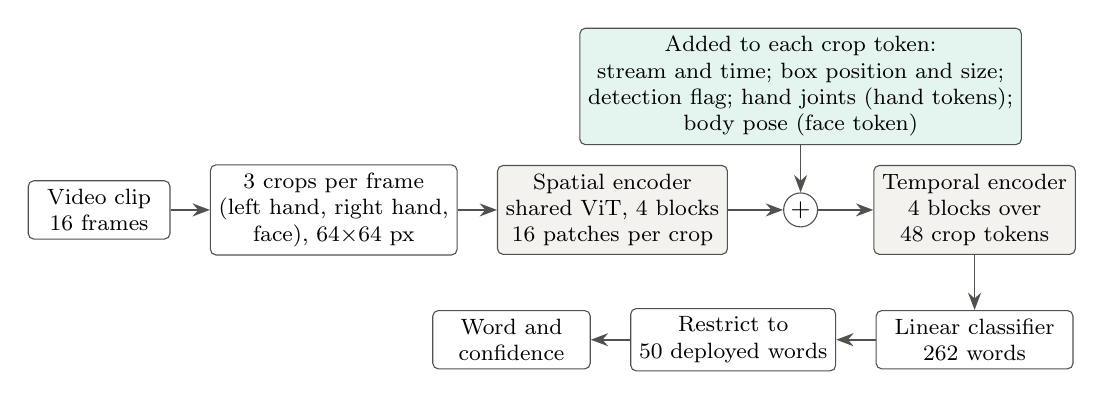
\begin{tikzpicture}[node distance=5mm and 5mm]
\node[box, minimum width=18mm] (in) {Video clip\\16 frames};
\node[box, right=of in, minimum width=27mm] (crops) {3 crops per frame\\(left hand, right hand,\\face), $64{\times}64$ px};
\node[stage, right=of crops, minimum width=25mm] (spat) {Spatial encoder\\shared ViT, 4 blocks\\16 patches per crop};
\node[circle, draw=ink2, inner sep=1pt, font=\small, right=7mm of spat] (plus) {$+$};
\node[box, above=6mm of plus, minimum width=44mm, fill=cC!12] (cond) {Added to each crop token:\\stream and time; box position and size;\\detection flag; hand joints (hand tokens);\\body pose (face token)};
\node[stage, right=7mm of plus, minimum width=25mm] (temp) {Temporal encoder\\4 blocks over\\48 crop tokens};
\node[box, below=7mm of temp, minimum width=25mm] (head) {Linear classifier\\262 words};
\node[box, left=of head, minimum width=25mm] (mask) {Restrict to\\50 deployed words};
\node[box, left=of mask, minimum width=20mm] (out) {Word and\\confidence};
\draw[arr] (in) -- (crops);
\draw[arr] (crops) -- (spat);
\draw[arr] (spat) -- (plus);
\draw[arr] (cond) -- (plus);
\draw[arr] (plus) -- (temp);
\draw[arr] (temp) -- (head);
\draw[arr] (head) -- (mask);
\draw[arr] (mask) -- (out);
\end{tikzpicture}}
\caption{ISL-ViT-Tiny. Attention is factorised: first within each crop, then across the 48 crop tokens of the clip.}\label{fig:model}
\begin{evidence}
\evitem{What it shows.} The computation graph of the released model. Shaded boxes are Transformer stacks; coloured boxes are the additive token-conditioning terms of Eq.~\eqref{eq:token}. The 50-word restriction is applied at prediction time only (Eq.~\eqref{eq:mask}).
\evitem{Evidence.} Model \ev{islvit/models/isl_vit.py\#L136-L299}{isl_vit.py:136-299}; landmark features \ev{islvit/models/isl_vit.py\#L312-L344}{isl_vit.py:312-344}; masking \ev{islvit/mask50.py\#L56-L108}{mask50.py:56-108}. Parameter counts were obtained by instantiating the model with \new{report/final/scripts/measure_model.py} (new in this report; output \new{report/final/data/model_measurements.json}).
\end{evidence}
\end{figure}

\subsection{Training procedure}\label{sec:method:train}
The released model was trained on the 2,845 training clips of the session-disjoint split with validation folded in (Section~\ref{sec:method:eval}), for a fixed 1,000 epochs, keeping the final weights (\ev{islvit/train.py\#L244-L730}{train.py:244}; launch scripts \ev{run_landmarks.sh}{run_landmarks.sh} and \ev{run_lm_s2_resume.sh}{run_lm_s2_resume.sh}). The optimiser is AdamW~\cite{loshchilov2019adamw} with a peak learning rate of $5\times10^{-4}$, 10 warm-up epochs, cosine decay to 1\%, batch 64 and weight decay 0.05 on weight matrices only; the spatial encoder learns at 0.1 times the base rate. Regularisation uses label smoothing of 0.1~\cite{szegedy2016inception}, mixup with $\alpha=0.2$ on half the batches~\cite{zhang2018mixup}, stochastic depth up to 0.1~\cite{huang2016stochdepth}, gradient clipping at 1.0 and an exponential moving average of the weights. Augmentation applies temporal jitter within uniform segments, scale-jittered crop windows, horizontal flips that swap the two hand streams and their joints, brightness, contrast and per-channel gain changes, greyscale, stream dropout, and a per-clip resolution jitter. Seeds 0, 1 and 2 give three independent models. The effective recipe of each run is stored in its \texttt{summary.json}.

Checkpoint selection on validation was abandoned because validation clips come from the training sessions. On the 262-word split, keeping the final weights instead of the best-validation checkpoint raised test top-1 from 22.1\% to 25.3\% (Table~\ref{tab:trace}, row E6).

\subsection{Self-supervised initialisation}\label{sec:method:ssl}
Both encoders are initialised from masked-image pretraining on iSign in the style of SimMIM~\cite{xie2022simmim} (\ev{islvit/pretrain.py\#L182-L258}{pretrain.py:182}; launch \ev{run_isign_pipeline.sh}{run_isign_pipeline.sh}). A learned mask token replaces 75\% of the patch tokens, sampled jointly over time, stream and space; a two-block decoder predicts per-patch-normalised pixels, and the loss is the mean squared error on masked patches. Interpolated crops are excluded from the loss so that the model does not learn to reconstruct stale background. Position and time embeddings are resized when the pretrained geometry differs from the fine-tuning geometry (\ev{islvit/train.py\#L75-L116}{train.py:75}).

\subsection{Four-bit quantisation}\label{sec:method:quant}
Every weight matrix (tensors with at least two dimensions) is split into groups $G$ of 128 consecutive weights and quantised symmetrically (\ev{islvit/export.py\#L223-L238}{export.py:223}):
\begin{equation}
\sigma_G=\operatorname{fp16}\!\Big(\frac{\max_{w\in G}|w|}{7}\Big),\qquad c_w=\operatorname{clamp}\big(\operatorname{round}(w/\sigma_G),-8,7\big),\qquad \hat{w}=\sigma_G\,c_w.\label{eq:int4}
\end{equation}
Two 4-bit codes are packed per byte with one FP16 scale per group; embeddings, normalisation parameters and biases stay in FP16 (\ev{islvit/export.py\#L202-L220}{export.py:202}, \ev{islvit/export.py\#L246-L294}{export.py:246}). Post-training quantisation (PTQ) applies Eq.~\eqref{eq:int4} to the trained FP32 weights (\ev{islvit/int4_eval.py}{int4_eval.py}). Quantisation-aware training (QAT) continues training for a fixed 300 epochs at a learning rate of $5\times10^{-5}$, computing the forward pass with $\hat{w}$ and applying the gradients to the full-precision weights, a straight-through estimator~\cite{bengio2013ste,jacob2018quant} implemented by swapping tensors around each step (\ev{islvit/qat.py\#L50-L84}{qat.py:50}; launch \ev{run_lm_qat.sh}{run_lm_qat.sh}). QAT and the exporter call the same target-selection and rounding functions, so the model trained is the model saved. An earlier pixel-only QAT run had chosen its epoch by test accuracy; it was withdrawn, and the landmark QAT was re-run with the final epoch fixed in advance. The release files are written by \ev{islvit/release.py}{release.py} and read by \ev{islvit/export.py\#L181-L200}{export.py:181}, which rebuilds FP32 weights from the codes. Inference arithmetic is therefore FP32: the 4-bit format reduces storage, not compute.

\subsection{Super-resolution front end and GAN study}\label{sec:method:sr}
For video below 720 pixels in height, the frame reader enlarges frames before detection. The default is bicubic interpolation; the alternative is a $\times4$ generator applied at the same point (\ev{islvit/data/crops.py\#L163-L204}{crops.py:163}). The generator is a compact VGG-style network of the kind distributed with the Real-ESRGAN code base, trained on Real-ESRGAN-style synthetic degradations~\cite{wang2021realesrgan}: 3$\times$3 convolutions at low resolution, a final pixel shuffle, and a residual over nearest-neighbour upsampling (\ev{islvit/sr/models.py\#L32-L48}{sr/models.py:32}). Training pairs come from high-resolution hand, face and frame patches of training sessions only, degraded by random blur, resizing, noise and JPEG compression (\ev{islvit/sr/degrade.py\#L122-L149}{sr/degrade.py:122}). Figure~\ref{fig:gan} shows the comparison design. The arms are:
\begin{itemize}
\item \textbf{SR-L1 (no GAN)}: a 621,424-parameter generator trained for 100,000 iterations with pixel L1 loss only.
\item \textbf{SR-GAN v1}: SR-L1 fine-tuned for 60,000 iterations with L1, VGG19 perceptual~\cite{johnson2016perceptual,simonyan2015vgg} and adversarial~\cite{goodfellow2014gan} losses against a spectrally normalised U-Net discriminator~\cite{schonfeld2020unetd,miyato2018sn} (\ev{islvit/sr/models.py\#L51-L81}{sr/models.py:51}). Its comparison with SR-L1 was pre-registered.
\item \textbf{SR-GAN v2}: v1 trained for 80,000 further iterations with a fresh discriminator; designed after v1's results were seen.
\item \textbf{SR-GAN v3 and its control}: a 2,039,568-parameter generator with a relativistic average adversarial loss~\cite{jolicoeur2019ragan}, H.264 degradation, and a loss on hand landmarks predicted by a differentiable ResNet-18~\cite{he2016resnet} heatmap network with soft-argmax readout~\cite{sun2018integral} (\ev{islvit/sr/train.py\#L100-L109}{sr/train.py:100}). The control is the same generator and hand loss without the discriminator. Designed after v1 and v2.
\end{itemize}
Test inputs are the 472 test clips degraded deterministically inside the frame reader by area downscaling and one JPEG encode: 360p (quality 60), 240p (50) and 180p (40) (\ev{islvit/sr/degrade.py\#L35-L43}{sr/degrade.py:35}; launch \ev{run_gan_study.sh}{run_gan_study.sh}, \ev{run_gan_study_v2.sh}{run_gan_study_v2.sh}, \ev{run_gan_v3_test.sh}{run_gan_v3_test.sh}). The three released classifiers are scored unchanged on each front end's output. Before the first test run, the rule for a verdict was fixed: ``helps'' requires a higher mean, all three seeds in the same direction, and pooled exact McNemar $p<0.05$ (\ev{islvit/gan_report.py\#L98-L117}{gan_report.py:98}).

\begin{figure}[t]
\centering
\resizebox{\linewidth}{!}{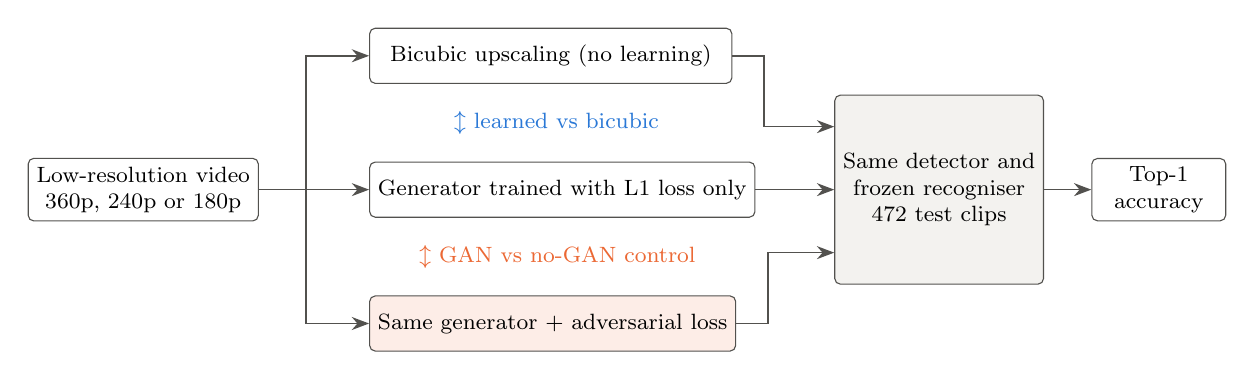
\begin{tikzpicture}[node distance=4mm and 6mm]
\node[box, minimum width=26mm] (lr) {Low-resolution video\\360p, 240p or 180p};
\node[box, right=14mm of lr, yshift=17mm, minimum width=46mm] (bic) {Bicubic upscaling (no learning)};
\node[box, right=14mm of lr, minimum width=46mm] (l1) {Generator trained with L1 loss only};
\node[box, right=14mm of lr, yshift=-17mm, minimum width=46mm, fill=cB!12] (gan) {Same generator + adversarial loss};
\node[font=\footnotesize, text=cA] at ($(bic.south)!0.5!(l1.north)$) {$\updownarrow$ learned vs bicubic};
\node[font=\footnotesize, text=cB] at ($(l1.south)!0.5!(gan.north)$) {$\updownarrow$ GAN vs no-GAN control};
\node[stage, right=10mm of l1, minimum width=26mm, minimum height=24mm] (rec) {Same detector and\\frozen recogniser\\472 test clips};
\node[box, right=6mm of rec, minimum width=17mm] (acc) {Top-1\\accuracy};
\draw[arr] (lr.east) -- ++(6mm,0) |- (bic.west);
\draw[arr] (lr.east) -- (l1.west);
\draw[arr] (lr.east) -- ++(6mm,0) |- (gan.west);
\draw[arr] (bic.east) -- ++(4mm,0) |- ([yshift=8mm]rec.west);
\draw[arr] (l1.east) -- (rec.west);
\draw[arr] (gan.east) -- ++(4mm,0) |- ([yshift=-8mm]rec.west);
\draw[arr] (rec) -- (acc);
\end{tikzpicture}}
\caption{Design of the super-resolution comparison. Only the upscaling step changes between arms.}\label{fig:gan}
\begin{evidence}
\evitem{What it shows.} The two comparisons the study makes. Bicubic versus a learned upscaler measures what learning to upscale buys; a GAN versus the same generator without the discriminator measures what the adversarial term buys. v3 has its own matched control (same generator and hand loss, no discriminator).
\evitem{Evidence.} Networks \ev{islvit/sr/models.py}{sr/models.py}; training \ev{islvit/sr/train.py\#L137-L382}{sr/train.py:137}; insertion point \ev{islvit/data/crops.py\#L163-L204}{crops.py:163}; drivers \ev{run_gan_study.sh}{run_gan_study.sh}, \ev{run_gan_v3.sh}{run_gan_v3.sh}. Generator weights are local only; their SHA-256 hashes are recorded in each test cache's front-end description, copied into \evdir{runs/gan_study/detection}{runs/gan_study/detection/*.json}.
\end{evidence}
\end{figure}

\subsection{Evaluation protocol}\label{sec:method:eval}
INCLUDE file names carry the camera's running clip counter (\texttt{MVI\_xxxx}). Clips of one word whose counters differ by at most 5 form a \emph{take-group} of back-to-back recordings (\ev{islvit/data/splits.py\#L118-L136}{splits.py:118}); the gap histogram is bimodal, and thresholds from 5 to 20 give the same partition. Clustering the counters of the whole corpus with the same gap gives 13 contiguous \emph{session blocks} (\ev{islvit/data/splits.py\#L170-L206}{splits.py:170}). The session-disjoint split assigns whole blocks to test by random search over 20,000 candidate assignments, scored mainly on how many test words keep at least six training clips (\ev{islvit/data/splits.py\#L209-L299}{splits.py:209}). Blocks 0, 5 and 6 form the test side. Figure~\ref{fig:protocols} contrasts the three protocols.

\begin{figure}[t]
\centering
\resizebox{\linewidth}{!}{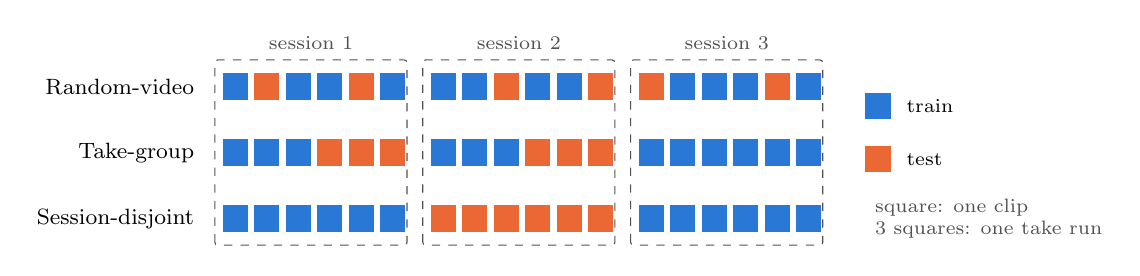
\begin{tikzpicture}[x=4.0mm, y=4.2mm]
\newcommand{\cliprow}[3]{%
  \node[anchor=east, font=\footnotesize, align=right] at (-0.6,#1) {#2};
  \foreach \i/\c in {#3} {\fill[\c] (\i,#1-0.4) rectangle (\i+0.8,#1+0.4);}
}
\foreach \x/\n in {0/1, 6.6/2, 13.2/3} {
  \draw[ink2, dashed, rounded corners=1pt] (\x-0.25,-2.8) rectangle (\x+5.85,2.8);
  \node[font=\scriptsize, text=ink2] at (\x+2.8,3.3) {session \n};
}
\cliprow{2}{Random-video}{0/cA,1/cB,2/cA,3/cA,4/cB,5/cA, 6.6/cA,7.6/cA,8.6/cB,9.6/cA,10.6/cA,11.6/cB, 13.2/cB,14.2/cA,15.2/cA,16.2/cA,17.2/cB,18.2/cA}
\cliprow{0}{Take-group}{0/cA,1/cA,2/cA,3/cB,4/cB,5/cB, 6.6/cA,7.6/cA,8.6/cA,9.6/cB,10.6/cB,11.6/cB, 13.2/cA,14.2/cA,15.2/cA,16.2/cA,17.2/cA,18.2/cA}
\cliprow{-2}{Session-disjoint}{0/cA,1/cA,2/cA,3/cA,4/cA,5/cA, 6.6/cB,7.6/cB,8.6/cB,9.6/cB,10.6/cB,11.6/cB, 13.2/cA,14.2/cA,15.2/cA,16.2/cA,17.2/cA,18.2/cA}
\fill[cA] (20.4,1.0) rectangle (21.2,1.8); \node[anchor=west, font=\scriptsize] at (21.4,1.4) {train};
\fill[cB] (20.4,-0.6) rectangle (21.2,0.2); \node[anchor=west, font=\scriptsize] at (21.4,-0.2) {test};
\node[anchor=west, font=\scriptsize, text=ink2, align=left] at (20.4,-2.0) {square: one clip\\3 squares: one take run};
\end{tikzpicture}}
\caption{Three split protocols on the same recordings. Each session holds several words, each recorded as a run of near-identical takes.}\label{fig:protocols}
\begin{evidence}
\evitem{What it shows.} A schematic, not data. Random-video splits put takes of one run on both sides; take-group splits keep a run together but let one session supply both training and test clips; session-disjoint splits hold out whole sessions.
\evitem{Measured on the split files.} With blocks rebuilt independently from file names (\new{report/final/scripts/audit_results.py}), the 262-word random-video split has 666 take-groups on both sides of the train/test boundary; the take-group split has all 13 blocks on both sides; the training split of the final models (\ev{splits/full263__session-disjoint-foldval.csv}{full263__session-disjoint-foldval.csv}) and the deployed split (\ev{splits/vocab50clean__session-disjoint.csv}{vocab50clean__session-disjoint.csv}) have none.
\evitem{What it does not show.} Session blocks are inferred from counters, not from signer identities, which INCLUDE does not publish. A held-out block may contain a signer who also appears in training blocks.
\end{evidence}
\end{figure}

For final models, the validation clips (taken from training sessions at take-group granularity) are folded back into training, giving 2,845 training clips over 262 words. The held-out blocks contain 1,412 clips: 1,010 form the test set, and 402 belong to words with fewer than six training clips and are marked unused. The deployed test set is the 472 test clips of the 50 deployed words (\ev{splits/_test472_paths.csv}{_test472_paths.csv}); the audit script confirmed that this list equals the test rows of the deployed split and that every headline result file scores exactly these clips.

\subsection{Metrics, test-time views and statistics}\label{sec:method:metrics}
Top-1 and top-5 accuracy are the share of clips whose true word is ranked first or within the first five; balanced accuracy is the mean per-word recall (\ev{islvit/tta.py\#L65-L75}{tta.py:65}). \emph{Masked-50} applies Eq.~\eqref{eq:mask} with $\mathcal{D}$ the deployed words; \emph{wide-262} takes the argmax over all 262 outputs. Test-time augmentation (TTA) averages softmax probabilities over six views: three temporal phases (0.25, 0.5 and 0.75 of each sampling segment), each with and without a horizontal flip that swaps the hand streams (\ev{islvit/tta.py\#L46-L62}{tta.py:46}). Each headline figure is the mean of three seeds; the best seed is never quoted. Paired comparisons on identical clips use the exact two-sided McNemar test~\cite{mcnemar1947} on the discordant clips, per seed and pooled over seeds. Five seeds of one earlier configuration gave a top-1 standard deviation of 1.9 points on 1,010 clips (\ev{runs/sd263_ssl_foldval/summary.json}{runs/sd263_ssl_foldval*}), so differences below about 5 points between single runs were treated as unresolved.

\subsection{Application path}\label{sec:method:app}
The application is a standard-library HTTP server (\ev{islvit/serve.py\#L102-L202}{serve.py:102}) and a seven-screen browser interface built into one page from \evdir{islvit/ui/src}{islvit/ui/src}. \texttt{POST /predict} receives raw video bytes and runs the same extraction, landmark and view functions as the offline evaluation (\ev{islvit/serve.py\#L50-L99}{serve.py:50}). The demo launcher (\ev{islvit/demo.py\#L69-L118}{demo.py:69}) replaces the server's classifier with one that applies the 50-word restriction exactly as in Eq.~\eqref{eq:mask}, and can bind a super-resolution generator into the frame reader. The model is chosen with \texttt{--run} at launch; the interface itself has no model selector. A prediction whose confidence is below a threshold $\tau$ (default 0.40) goes to a screen listing five candidates, and a user's correction is appended to a log. Figure~\ref{fig:system} shows the offline and online paths.

\begin{figure}[t]
\centering
\resizebox{\linewidth}{!}{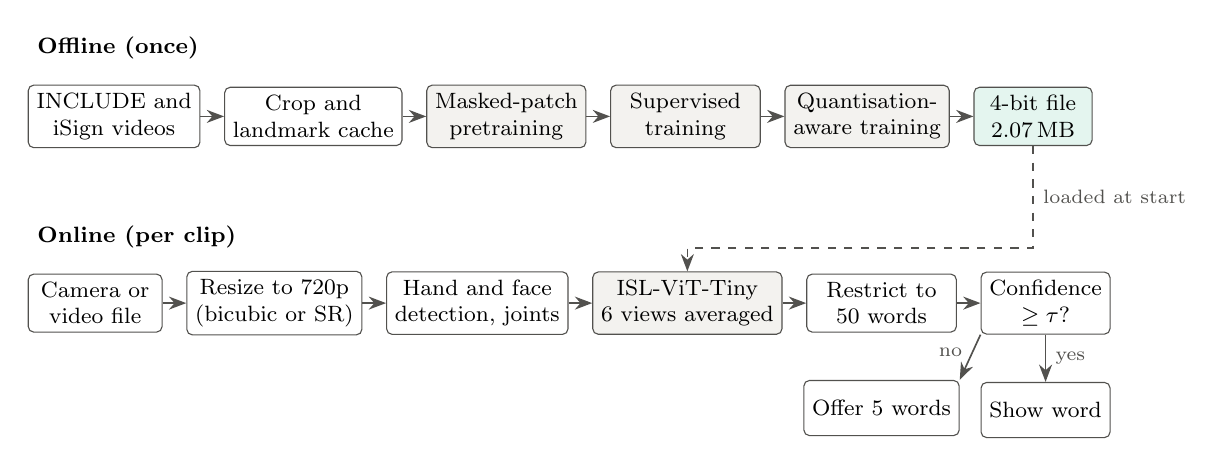
\begin{tikzpicture}[node distance=3mm and 3mm]
\node[font=\footnotesize\bfseries, anchor=west] (offt) at (0,0) {Offline (once)};
\node[box, below=2mm of offt.south west, anchor=north west, minimum width=17mm] (o1) {INCLUDE and\\iSign videos};
\node[box, right=of o1, minimum width=18mm] (o2) {Crop and\\landmark cache};
\node[stage, right=of o2, minimum width=19mm] (o3) {Masked-patch\\pretraining};
\node[stage, right=of o3, minimum width=19mm] (o4) {Supervised\\training};
\node[stage, right=of o4, minimum width=19mm] (o5) {Quantisation-\\aware training};
\node[box, right=of o5, minimum width=15mm, fill=cC!12] (o6) {4-bit file\\2.07\,MB};
\foreach \a/\b in {o1/o2,o2/o3,o3/o4,o4/o5,o5/o6} \draw[arr] (\a) -- (\b);
\node[font=\footnotesize\bfseries, anchor=west] (ont) at (0,-2.4) {Online (per clip)};
\node[box, below=2mm of ont.south west, anchor=north west, minimum width=17mm] (n1) {Camera or\\video file};
\node[box, right=of n1, minimum width=18mm] (n2) {Resize to 720p\\(bicubic or SR)};
\node[box, right=of n2, minimum width=19mm] (n3) {Hand and face\\detection, joints};
\node[stage, right=of n3, minimum width=19mm] (n4) {ISL-ViT-Tiny\\6 views averaged};
\node[box, right=of n4, minimum width=19mm] (n5) {Restrict to\\50 words};
\node[box, right=of n5, minimum width=15mm] (n6) {Confidence\\$\ge\tau$?};
\foreach \a/\b in {n1/n2,n2/n3,n3/n4,n4/n5,n5/n6} \draw[arr] (\a) -- (\b);
\node[box, below=6mm of n5, minimum width=15mm] (no) {Offer 5 words};
\node[box, below=6mm of n6, minimum width=15mm] (yes) {Show word};
\draw[arr] (n6) -- node[lab, right]{yes} (yes);
\draw[arr] (n6.south west) -- node[lab, left, pos=0.4]{no} (no.north east);
\draw[arr, dashed] (o6.south) |- node[lab, pos=0.25, right]{loaded at start} ([yshift=3mm]n4.north) -- (n4.north);
\end{tikzpicture}}
\caption{End-to-end system: offline training and compression, and the per-clip inference path shared by the evaluation and the application.}\label{fig:system}
\begin{evidence}
\evitem{What it shows.} Shaded boxes are learned stages. The online path is shared by the offline test cache and the server: \ev{islvit/predict.py\#L42-L107}{predict.py:42-107}, \ev{islvit/serve.py\#L50-L99}{serve.py:50-99}, \ev{islvit/demo.py\#L69-L118}{demo.py:69-118}. Training commands: \ev{run_isign_pipeline.sh}{run_isign_pipeline.sh} (pretraining), \ev{run_landmarks.sh}{run_landmarks.sh} (supervised), \ev{run_lm_qat.sh}{run_lm_qat.sh} (QAT), \ev{islvit/release.py}{release.py} (release file).
\end{evidence}
\end{figure}

\subsection{Software and hardware}
Experiments ran on one desktop: NVIDIA GeForce RTX 3060 (12\,GB), AMD Ryzen 5 5500, 32\,GB RAM, Windows 11, Python 3.11.15, PyTorch 2.6.0 with CUDA 12.4, MediaPipe 1.0.0 (Tasks API), timm 1.0.28 and OpenCV. Training seeds were 0, 1 and 2; split construction used seed 1337.

% ===========================================================================
\section{Experimental setup}\label{sec:setup}
% ===========================================================================

Table~\ref{tab:setup} lists the settings of the principal experiments. All results in Sections~\ref{sec:res:main} to~\ref{sec:res:perclass} use the same 472 test clips unless the table says otherwise; experiments on other test sets are reported separately and are not ranked against the headline. Appendix~\ref{app:trace} links each experiment to its launch script and result files.

\begin{table}[t]
\caption{Settings of the principal experiments.}\label{tab:setup}
\scriptsize
\setlength{\tabcolsep}{3pt}
\begin{tabularx}{\textwidth}{@{}L{2.3cm}YL{2.6cm}L{1.4cm}L{2.0cm}@{}}
\toprule
Experiment & Models compared & Test set & Seeds & Metric \\
\midrule
Main result and variants & pixel FP32; landmark FP32; landmark PTQ INT4; landmark QAT INT4 (released) & 472 clips, 50 words, held-out sessions & 3 each & masked-50, 6-view TTA \\
Protocol comparison & one 50-word pixel recipe on random-video and session-disjoint splits & 200 and 472 clips (different sets) & 1 and 2 & top-1, single view \\
Temporal length & 8, 16, 24, 32 frames from one 32-frame cache, 50-word pixel recipe & 472 clips & 1 (16 frames: 2) & top-1, single view and TTA \\
Crop resolution & 64, 112, 128 pixel input, early 8-frame recipe & INCLUDE-50 take-group, 159 clips & 1 & top-1 \\
Cross-corpus & INCLUDE-trained models on CISLR & 609 CISLR clips & 1 to 3 & top-1 \\
Super-resolution & bicubic, SR-L1, SR-GAN v1, v2, v3, v3 control; frozen INT4 classifiers & 472 clips degraded to 360p, 240p, 180p & 3 & masked-50, TTA; McNemar \\
Application route & INT4 landmark, FP32 landmark, FP32 pixel (seed 0); INT4 with bicubic, SR-L1 and SR-GAN v2 at 180p; all through \texttt{POST /predict} & 50 of the 472 clips (one per word) & 1 & agreement with offline outcome \\
\botrule
\end{tabularx}
\end{table}

% ===========================================================================
\section{Results}\label{sec:results}
% ===========================================================================

\subsection{Main result}\label{sec:res:main}

\begin{evidence}
\evitem{Observed.} The released 4-bit landmark model reached 85.9\% top-1 (seeds 84.5, 87.5 and 85.8), 96.4\% top-5 and 85.8\% balanced accuracy.
\evitem{How measured.} Masked-50 with six-view TTA on the 472 held-out-session test clips; mean of three independently trained seeds; test cache extracted with a freshly built detector per video.
\evitem{Comparison.} Answering from all 262 words gives 72.0\% top-1 (69.7, 75.8, 70.3) and 92.7\% top-5 on the same clips; a single centre view with the mask gives 85.5\%.
\evitem{Evidence.} \ev{runs/f16_262w_lm_s0_qat4/masked50_clean.json}{runs/f16_262w_lm_s*_qat4/masked50_clean.json} (keys \texttt{masked\_tta}, \texttt{wide\_tta}, \texttt{masked\_plain}); evaluator \ev{islvit/mask50.py\#L56-L108}{mask50.py:56}; split \ev{splits/vocab50clean__session-disjoint.csv}{vocab50clean__session-disjoint.csv}. During this audit we re-scored the three files in \evdir{release}{release/} on the local test cache; per-clip outcomes matched the tracked files exactly for all three seeds (\new{report/final/audit/rescore_release_s*.json}).
\evitem{Interpretation.} The figure describes 50 words of INCLUDE studio video from held-out sessions. It does not describe the 262-word task (64.7\% top-1 on all 1,010 test clips, single view, from each QAT run's \texttt{summary.json}), other corpora (Section~\ref{sec:res:cross}) or new signers.
\end{evidence}

\subsection{Model variants}\label{sec:res:variants}

The repository contains one architecture family. Its variants differ in input streams, numerical precision, temporal length and preprocessing, not in network type; no CNN, recurrent or 3D-convolutional baseline was trained on the project's split. Table~\ref{tab:variants} and Fig.~\ref{fig:variants} compare the four variants that share the test set, the training data and the recipe.

\begin{table}[t]
\caption{Controlled variants on the 472 held-out clips (masked-50, 6-view TTA, mean of three seeds). Each row changes one thing relative to the row above it.}\label{tab:variants}
\footnotesize
\setlength{\tabcolsep}{4pt}
\begin{tabular*}{\textwidth}{@{\extracolsep\fill}llrrrrr@{}}
\toprule
Variant & Precision & Parameters & Stored size & Top-1 & Top-5 & Balanced \\
\midrule
Pixels only & FP32 & 3,803,206 & 15.2\,MB$^{a}$ & 73.7 & 93.5 & 73.3 \\
Pixels + landmarks & FP32 & 3,894,214 & 15.6\,MB$^{a}$ & 86.5 & 96.5 & 86.5 \\
Landmarks, PTQ & INT4, group 128 & 3,894,214 & as QAT$^{b}$ & 83.4 & 95.8 & 83.3 \\
Landmarks, QAT (released) & INT4, group 128 & 3,894,214 & 2,069,700\,B & 85.9 & 96.4 & 85.8 \\
\botrule
\end{tabular*}
\footnotetext{Per-seed top-1: pixels only 75.0/73.7/72.2; landmarks 87.3/86.9/85.4; PTQ 83.1/85.2/82.0; QAT 84.5/87.5/85.8. $^{a}$Parameters $\times$ 4 bytes, not a measured file. $^{b}$Same packing as the released file; no PTQ release file was written. 2,069,700\,B = 1.974\,MiB = 2.07\,MB.}
\end{table}

\begin{figure}[t]
\centering
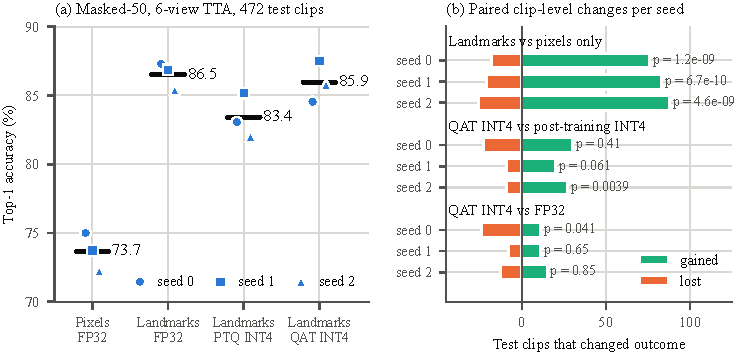
\includegraphics[width=\textwidth]{figures/fig_variants.pdf}
\caption{Controlled variant comparison on the deployed test set.}\label{fig:variants}
\begin{evidence}
\evitem{What it shows.} (a) Top-1 accuracy of each seed (markers) and the three-seed mean (bar). (b) For each seed, the test clips that the second model gets right and the first gets wrong (gained) or the reverse (lost), with the exact McNemar $p$ for that seed.
\evitem{Data.} \ev{runs/f16_262w_s0/masked50_clean.json}{runs/f16_262w_s*/masked50_clean.json}, \ev{runs/f16_262w_lm_s0/masked50_clean.json}{runs/f16_262w_lm_s*/masked50_clean.json}, \ev{runs/f16_262w_lm_s0/ptq4_clean.json}{runs/f16_262w_lm_s*/ptq4_clean.json}, \ev{runs/f16_262w_lm_s0_qat4/masked50_clean.json}{runs/f16_262w_lm_s*_qat4/masked50_clean.json}; keys \texttt{masked\_tta.top1} and \texttt{hits\_masked\_tta}. Training: \ev{run_landmarks.sh}{run_landmarks.sh}, \ev{run_lm_qat.sh}{run_lm_qat.sh}. Statistics and plot: \new{report/final/scripts/audit_results.py} and \new{make_figures.py} (new).
\end{evidence}
\end{figure}

\paragraph{Landmark stream.} Adding the landmark stream, with nothing else changed, raised top-1 from 73.7\% to 86.5\%. The gain replicated in every seed: 76, 83 and 88 clips gained against 18, 21 and 26 lost ($p=1.2\times10^{-9}$, $6.7\times10^{-10}$ and $4.6\times10^{-9}$). The pipeline already ran MediaPipe to place crop boxes; the landmark model uses joints that the pixel-only model discarded.

\paragraph{Quantisation.} Rounding the FP32 landmark weights to 4 bits after training lost 3.1 points (86.5\% to 83.4\%); quantisation-aware training reached 85.9\%. Pooled over seeds, QAT gained 77 clips and lost 41 relative to PTQ ($p=0.0012$), although only seed 2 reached $p<0.05$ on its own. Against FP32, QAT gained 37 clips and lost 45 (pooled $p=0.44$), so three seeds do not resolve a difference between the released 4-bit model and its FP32 parent; seed 0 alone lost significantly (11 gained, 24 lost, $p=0.041$).

\paragraph{Compute and latency.} Table~\ref{tab:runtime} reports measurements made for this report. Model-only CPU latency was \LATMS\ per view. The end-to-end server route, which decodes a 1080p clip and runs MediaPipe twice over 32 frames, took a median of 4.3\,s per clip on the same CPU, so detection and decoding, not the Transformer, dominate the end-to-end time.

\begin{table}[t]
\caption{Compute and runtime of the released model, measured during this audit on the desktop described in Section~\ref{sec:method}. Nothing was measured on a phone or wearable device.}\label{tab:runtime}
\footnotesize
\setlength{\tabcolsep}{4pt}
\begin{tabularx}{\textwidth}{@{}L{3.4cm}L{2.7cm}Y@{}}
\toprule
Quantity & Value & Timing boundary and method \\
\midrule
Parameters (landmark model, 262 outputs) & 3,894,214 & counted on the instantiated network; spatial encoder 1,930,944, temporal blocks 1,779,456, landmark projections 91,008 \\
Multiply--accumulates per view & 1.65\,G (16 frames); 0.82\,G (8 frames) & \texttt{torch.utils.flop\_counter}; matrix products and convolutions only \\
Model forward pass, one view, CPU & \LATMS\ median (IQR \LATIQR) & released seed-0 file, batch 1, FP32 arithmetic after dequantisation, 6 threads, 100 runs after warm-up, idle machine \\
Server route, one clip, CPU & 4.3\,s median (10 clips) & \texttt{POST /predict} on a 1080p source: decoding, detection and landmarks, 6 views, 50-word mask \\
Server route, one clip, GPU & 3.7\,s median (50 clips) & as above, model and detector on the RTX 3060 \\
\botrule
\end{tabularx}
\footnotetext{Sources: \new{report/final/data/model_measurements.json} (\new{measure_model.py}); \new{report/final/data/app_integration_int4_lm_s0.json} and \new{app_integration_int4_lm_s0_cpu.json} (\new{app_integration_test.py}).}
\end{table}

\subsection{Effect of the split protocol}\label{sec:res:protocol}

\begin{figure}[t]
\centering
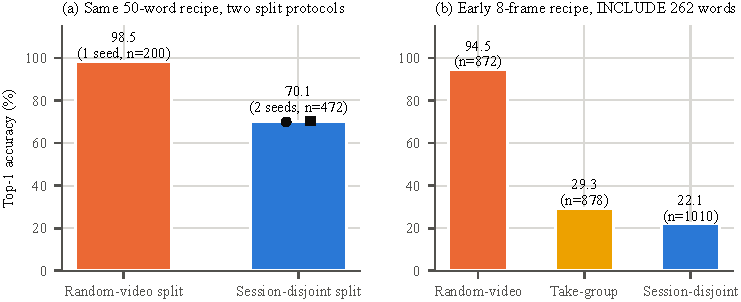
\includegraphics[width=\textwidth]{figures/fig_protocol.pdf}
\caption{Accuracy of one recipe under different split protocols.}\label{fig:protocol}
\begin{evidence}
\evitem{What it shows.} (a) A 50-word pixel-only recipe (16 frames, 2,000 epochs, iSign initialisation) trained on a random-video split and on the session-disjoint split. (b) An early 8-frame, 262-word recipe trained on three split files. Labels give the test-set size $n$; the bars do not share a test set, because each protocol defines its own.
\evitem{Data.} (a) \ev{runs/baseline_random_s0/summary.json}{runs/baseline_random_s0}, \ev{runs/f16_clean_s0/summary.json}{runs/f16_clean_s0}, \ev{runs/f16_clean_s1/summary.json}{runs/f16_clean_s1} (key \texttt{test.top1}); splits \ev{splits/vocab50__random-video.csv}{vocab50__random-video.csv} and \ev{splits/vocab50clean__session-disjoint.csv}{vocab50clean__session-disjoint.csv}. (b) \ev{runs/full263_v2__random-video/summary.json}{runs/full263_v2__random-video}, \ev{runs/full263_v2__take-group/summary.json}{runs/full263_v2__take-group}, \ev{runs/sd_full263/summary.json}{runs/sd_full263}; launch \ev{run_phase2.sh}{run_phase2.sh}.
\evitem{Interpretation.} The random-video score is mostly recognition of the recording; the take-group step removes near-duplicate takes and the session step removes shared recording conditions. The 50-word comparison has one random-split seed and different test clips, so the 28-point gap is an estimate of size, not a paired measurement.
\end{evidence}
\end{figure}

The matched 50-word comparison gave 98.5\% on the random-video split (one seed, 200 clips) and 70.1\% on held-out sessions (69.9\% and 70.3\%, two seeds, 472 clips), a gap of 28.4 points. Earlier project documents paired the 98.5\% with a different 262-word model scored at 75.6\%; that pairing understated the gap and has been corrected in the repository (Appendix~\ref{app:disc}). With the early 8-frame recipe on 262 words, accuracy fell from 94.5\% (random-video) to 29.3\% (take-group) and 22.1\% (session-disjoint).

\subsection{Temporal length, resolution and training budget}\label{sec:res:ablation}

\begin{figure}[t]
\centering
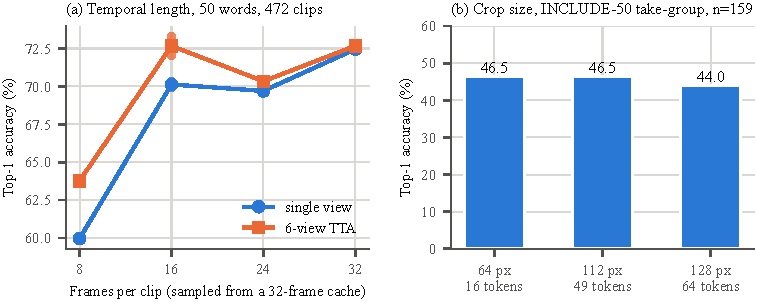
\includegraphics[width=\textwidth]{figures/fig_ablation.pdf}
\caption{Temporal length and crop resolution.}\label{fig:ablation}
\begin{evidence}
\evitem{What it shows.} (a) Top-1 of the 50-word pixel-only recipe with 8, 16, 24 or 32 frames sampled from the same 32-frame cache, single view and six-view TTA; at 16 frames the line is the mean of two seeds (dots). (b) Top-1 at three crop sizes, early 8-frame recipe, INCLUDE-50 take-group split (159 clips, one seed).
\evitem{Data.} (a) \ev{runs/f8_clean_s0/summary.json}{runs/f8_clean_s0}, \ev{runs/f16_clean_s0/summary.json}{f16_clean_s0}, \ev{runs/f16_clean_s1/summary.json}{f16_clean_s1}, \ev{runs/f24_clean_s0/summary.json}{f24_clean_s0}, \ev{runs/f32_clean_s0/summary.json}{f32_clean_s0} (keys \texttt{test}, \texttt{test\_tta}); launch \ev{run_frames32.sh}{run_frames32.sh}. (b) \ev{runs/abl64__take-group/summary.json}{runs/abl64__take-group}, \ev{runs/abl112__take-group/summary.json}{abl112__take-group}, \ev{runs/abl128__take-group/summary.json}{abl128__take-group}; launch \ev{run_ablation_res.sh}{run_ablation_res.sh}.
\end{evidence}
\end{figure}

Going from 8 to 16 frames raised single-view top-1 from 60.0\% to 70.1\% (two-seed mean); 24 and 32 frames gave 69.7\% and 72.5\% from one seed each, within the noise floor of the 16-frame result. The model uses 16 frames because 32 doubles inference cost without a resolved gain. Larger crops did not help: 64, 112 and 128 pixels gave 46.5\%, 46.5\% and 44.0\% at 0.82, 2.34 and 3.03 GMACs per view (measured with \new{measure_model.py}). On the 50-word tier, with a training split that also contained 76 CISLR clips and the same 472 test clips, extending training from 250 to 2,000 epochs raised top-1 by 7.9 points (two runs each; \ev{run_longtrain.sh}{run_longtrain.sh}, \ev{run_grokking.sh}{run_grokking.sh}). At 16 frames a 4,000-epoch run gained 0.6 points over 2,000 epochs, below the noise floor. Fine-tuning the 262-word model on the 50-word softmax moved the three seeds in opposite directions (75.6$\to$78.4, 73.5$\to$73.1 and 72.0$\to$68.4) and was rejected. Five further landmark variants (joint augmentation, gap interpolation, velocity, two-hand relation and wrist trajectory), screened on 154 validation clips, produced no variant that replicated across seeds, and none was adopted.

\subsection{Per-word behaviour}\label{sec:res:perclass}

\begin{figure}[t]
\centering
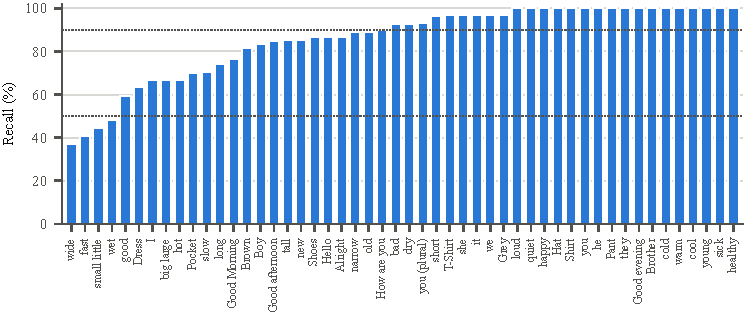
\includegraphics[width=\textwidth]{figures/fig_perclass.pdf}
\caption{Per-word recall of the released model on the 472 test clips.}\label{fig:perclass}
\begin{evidence}
\evitem{What it shows.} Recall per deployed word, pooled over the three released seeds (about 9 to 11 test clips per word per seed), sorted. Dotted lines mark 50\% and 90\%.
\evitem{Data.} \texttt{hits\_masked\_tta} and \texttt{video\_paths} in \ev{runs/f16_262w_lm_s0_qat4/masked50_clean.json}{runs/f16_262w_lm_s*_qat4/masked50_clean.json}; computed by \new{make_figures.py}.
\end{evidence}
\end{figure}

Twenty-seven of the 50 words reached at least 90\% recall. Four fell below 50\%: \emph{wide} (37.0\%), \emph{fast} (40.7\%), \emph{small} (44.4\%) and \emph{wet} (48.1\%). An earlier error analysis on validation clips, recorded in commit \texttt{42080f0} rather than in a result file, found that about 70\% of errors fell in six look-alike groups (for example \emph{big}/\emph{wide}/\emph{narrow} and \emph{good}/\emph{bad}/\emph{wet}) that differ mainly in movement or in the relation between the two hands; the levers aimed at those cues are the ones that failed screening.

\subsection{Cross-corpus test}\label{sec:res:cross}
INCLUDE-trained checkpoints from an earlier stage of the project (pixel-only, 8 frames) scored 41.8 to 42.4\% on the 1,010 INCLUDE test clips and 0.3 to 1.8\% on 609 CISLR clips, where chance is 0.38\% (\ev{crosscorpus_eval.log}{crosscorpus_eval.log}; launch \ev{run_crosscorpus_eval.sh}{run_crosscorpus_eval.sh}). Those checkpoints are not the released model. During this audit we extracted landmarks for the CISLR clips and scored the three released files (\new{report/final/scripts/run_crosscorpus_release.sh}): \CISLRRESULT. MediaPipe found a genuine left hand in 25.0\% of CISLR frames against 92.0\% on the 472 INCLUDE test clips (\ev{runs/gan_study/detection/cislr_bicubic.json}{runs/gan_study/detection/cislr_bicubic.json}), so part of the failure lies in detection on CISLR's 300-pixel video.

\subsection{Super-resolution and the GAN}\label{sec:res:gan}

\begin{figure}[p]
\centering
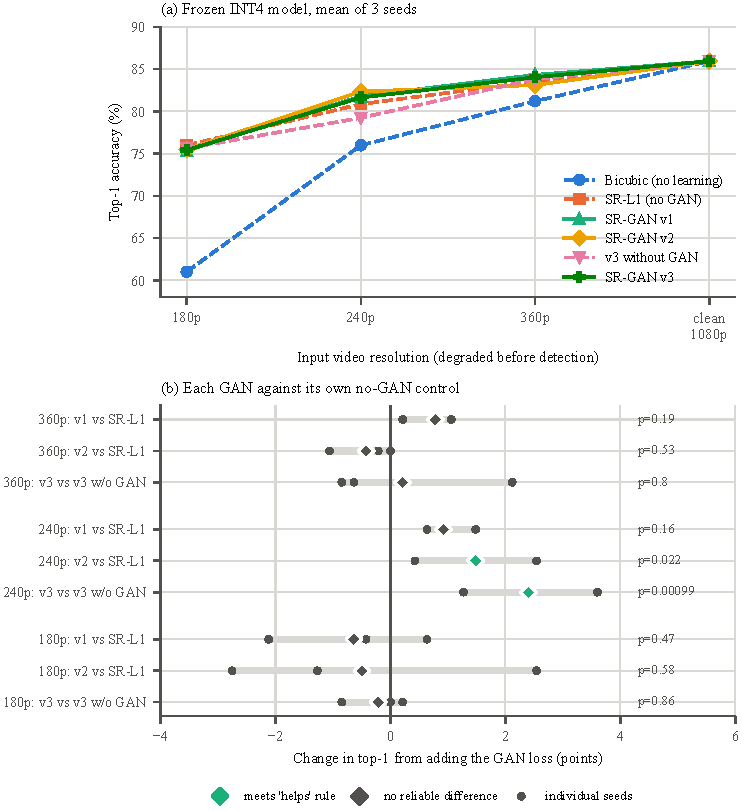
\includegraphics[width=\textwidth]{figures/fig_gan.pdf}
\caption{Learned upscaling versus bicubic, and each GAN versus its own no-GAN control.}\label{fig:ganres}
\begin{evidence}
\evitem{What it shows.} (a) Mean top-1 of the three frozen released models on the 472 test clips after each front end; dashed lines are arms without an adversarial loss, and clean 1080p is the headline 85.9\%. (b) Change in top-1 when the adversarial loss is added to an otherwise identical generator: diamonds are three-seed means, dots individual seeds, and $p$ is the pooled exact McNemar test.
\evitem{Data.} \evdir{runs/gan_study/frozen_int4}{runs/gan_study/frozen_int4/} and \evdir{runs/gan_study_v1/frozen_int4}{runs/gan_study_v1/frozen_int4/} (keys \texttt{masked\_tta.top1}, \texttt{hits\_masked\_tta}). The original verdicts come from \ev{islvit/gan_report.py\#L98-L117}{gan_report.py:98}; \new{audit_results.py} recomputed them with a separate implementation and agreed on every cell.
\end{evidence}
\end{figure}

\begin{table}[t]
\caption{Super-resolution study at 180p (frozen INT4 models, 472 clips, three seeds). Detection is the share of frames with a genuine left-hand detection; on the clean test cache it is 92.0\%. Image quality is measured on 1,200 held-out patches.}\label{tab:gan}
\footnotesize
\setlength{\tabcolsep}{4pt}
\begin{tabular*}{\textwidth}{@{\extracolsep\fill}lccccc@{}}
\toprule
Front end & GAN loss & Top-1 (\%) & Left hand found (\%) & PSNR (dB) & SSIM \\
\midrule
Bicubic & -- & 61.0 & 51.0 & 30.07 & 0.856 \\
SR-L1 & no & 76.0 & 68.2 & 31.83 & 0.900 \\
SR-GAN v1 & yes & 75.4 & 67.9 & 31.07 & 0.883 \\
SR-GAN v2 & yes & 75.5 & 68.6 & 31.09 & 0.884 \\
v3 without GAN & no & 75.6 & 65.5 & 29.96 & 0.863 \\
SR-GAN v3 & yes & 75.4 & 77.6 & 29.76 & 0.870 \\
\botrule
\end{tabular*}
\footnotetext{Sources: \new{runs/gan_study/frozen_int4/L3_*.json} and \new{runs/gan_study_v1/frozen_int4/L3_*.json}; \new{runs/gan_study/detection/L3_*.json} and \new{runs/gan_study_v1/detection/L3_srgan.json} (\texttt{streams.left\_hand.genuine}); \new{runs/gan_study/sr_quality*.json} and \new{runs/gan_study_v1/sr_quality.json} (level \texttt{L3 180p}).}
\end{table}

Every learned upscaler beat bicubic at every resolution; at 180p the gain was 14.3 to 15.0 points (SR-L1: +15.0, 269 clips gained and 57 lost, $p=4.5\times10^{-34}$). The adversarial loss is a different matter. Of the nine GAN-versus-control comparisons (three GANs at three resolutions), two met the pre-registered ``helps'' rule, both at 240p: v2 over SR-L1 (+1.5 points, $p=0.022$) and v3 over its control (+2.4, $p=0.001$). The second is weaker than it looks, because v3's control was the weakest learned front end at 240p and SR-GAN v3 did not beat SR-L1 there (+0.8, $p=0.30$). Training v1 longer into v2 lost 1.2 points at 360p ($p=0.021$). SR-GAN v3 found the most hands at 180p (77.6\% of frames against 68.2\% for SR-L1), yet its accuracy matched SR-L1's, so better detection statistics did not translate into better recognition by the frozen classifier. In line with the perception--distortion trade-off~\cite{blau2018pd}, the GANs produced sharper patches with lower PSNR than SR-L1.

After the classifiers were fine-tuned for 150 epochs on 360p video through each front end, GAN front ends still beat bicubic at 180p (v1 77.8\%, v2 76.9\%, bicubic 64.4\%). No fine-tuned SR-L1 arm exists, so these results cannot separate the adversarial term from learned upscaling. A 2$\times$2 decomposition at 180p with SR-GAN v2, crossing clean or degraded pixels with clean or degraded landmarks, attributed 7.7 of the 10.5 missing points to degraded landmarks and 2.9 to degraded pixels; the two parts need not sum to the total (\evdir{runs/gan_study/diagnostics}{runs/gan_study/diagnostics/}).

\subsection{Application integration and testing}\label{sec:res:app}

Table~\ref{tab:ui} separates four levels of evidence for each model: implemented, reachable through the application, tested through the application, and benchmarked on the full test set.

\begin{table}[t]
\caption{Integration status of each model variant.}\label{tab:ui}
\scriptsize
\setlength{\tabcolsep}{3pt}
\begin{tabularx}{\textwidth}{@{}L{2.8cm}L{1.3cm}L{2.5cm}YL{1.6cm}@{}}
\toprule
Model & Implemented & Reachable in the app & Tested through the app (this audit) & Benchmarked (472 clips) \\
\midrule
Landmark QAT INT4 (released, seed 0) & yes & default \texttt{--run} & 50 clips: 43 correct, 48 in top five; 50 of 50 outcomes match offline & yes, 3 seeds \\
Landmark FP32 (seed 0) & yes & \nolinkurl{--run runs/f16_262w_lm_s0} & 50 clips: 43 correct; 50 of 50 match offline & yes, 3 seeds \\
Pixels-only FP32 (seed 0) & yes & \nolinkurl{--run runs/f16_262w_s0} & 50 clips: 35 correct; 50 of 50 match offline & yes, 3 seeds \\
Landmark PTQ INT4 & yes & no release file & not tested & yes, 3 seeds \\
SR-L1 and SR-GAN v2 front ends & yes & \texttt{--sr} generator & \SRAPPRESULT & yes, 3 seeds \\
SR-GAN v1 and v3 front ends & yes & \texttt{--sr} generator & not tested & yes, 3 seeds \\
\botrule
\end{tabularx}
\footnotetext{Each app test posts raw video to \texttt{POST /predict} on the server started by \texttt{islvit.demo} and compares the top word with the same model's per-clip outcome in its \texttt{masked50\_clean.json}. The 50 clips are the first test clip of each deployed word. Script \new{report/final/scripts/app_integration_test.py}; outputs \new{report/final/data/app_integration_*.json}. Weights under \texttt{runs/} are local; only \texttt{release/} is public.}
\end{table}

For each of the three classifiers, all 50 server answers had the same correctness as the offline evaluation of that model on that clip, including the clips the model gets wrong. The application therefore runs the evaluated computation: the same detector settings, 16 of 32 frames, six views and the 50-word restriction. The same held for the super-resolution front end: with the 50 clips degraded to 180p (stored losslessly so that no second codec is added; \new{report/final/scripts/make_degraded_clips.py}), the server's answers through bicubic, SR-L1 and SR-GAN v2 matched the study's seed-0 outcomes on every clip, and the ordering on these clips (SR-L1 39, SR-GAN v2 37, bicubic 32 correct) follows the full study. The browser screens were not driven automatically in this audit. Earlier project records describe a Playwright check of all seven screens and live posting of ten demonstration clips, but the harness was not committed, so those outcomes rest on prose alone. The threshold curve on the Settings screen comes from an older pixel-only ensemble (88.7\% accuracy at 75.2\% coverage for $\tau=0.4$; \ev{runs/gate_mixed.json}{runs/gate_mixed.json}) and has not been re-measured for the released model.

\clearpage
% ===========================================================================
\section{Discussion and originality}\label{sec:discussion}
% ===========================================================================

\paragraph{What moved accuracy.} The largest single gain came from an input the pipeline already computed: hand joints added 12.8 points for 91,008 parameters. Doubling the frames from 8 to 16 added about 10 points, and training longer helped until 16 frames, then saturated. Larger crops, a narrower training objective and five landmark-derived features did not help. One reading is that with about 11 training clips per deployed word (571 clips for 50 words), explicit handshape measurements give the network information it cannot learn reliably from 64-pixel crops, while extra tokens and pixels mainly add ways to overfit. We did not test this explanation directly.

\paragraph{What compression costs.} Group-wise 4-bit storage reduces the weights from about 15.6\,MB to 2.07\,MB. Rounding after training cost 3.1 points; training with the rounding in the loop left a gap to FP32 that three seeds do not resolve. The released file is a storage format. The server rebuilds FP32 weights at load time, so the 4-bit model does not yet reduce arithmetic or memory traffic during inference.

\paragraph{What the protocol changes.} A 28-point gap between random-video and session-disjoint splits for one recipe means that INCLUDE accuracies reported on random splits largely measure recognition within recording sessions. Our 85.9\% figure sits below published INCLUDE-50 numbers~\cite{sridhar2020include,selvaraj2022openhands} at least partly because it is measured on a harder split; the two sets of numbers cannot be ranked against each other, and ours is not evidence of signer independence.

\paragraph{What the GAN study shows.} Learned upscaling recovered most of the accuracy lost at 180p, and the adversarial term added little on top of it. The 2$\times$2 decomposition suggests a reason: after upscaling, most of the remaining error lies in where the detector places hand joints, which texture realism does not target. The v3 generator, trained against a hand-landmark loss, improved detection statistics but not the frozen classifier's accuracy.

\paragraph{Originality.} We separate three kinds of claim. \emph{Algorithmic novelty}: none is claimed. Factorised video Transformers, masked-image pretraining, MediaPipe landmarks, straight-through quantisation, group-wise scales and GAN super-resolution are all prior work. \emph{System-level originality}: a region-crop factorised Transformer with additive position, detection-status and landmark conditioning, sized and quantised to a 2\,MB file, and served by an application that runs the evaluated code path. \emph{Experimental contribution}: seed-replicated, controlled measurements of each design lever on one locked test set; a session-aware split with a measured leakage gap; a cross-corpus drop (85.9\% to 29.3\%) reported rather than omitted; and a GAN study with a no-GAN control. Table~\ref{tab:contrib} ties each claim to its evidence. Among the works reviewed in Section~\ref{sec:related} we found no ISL word recogniser that reports these properties together; the search was limited to those sources, and the claim should be read in that scope.

\begin{sidewaystable}
\caption{Claimed contributions, closest prior approach and evidence.}\label{tab:contrib}
\scriptsize
\setlength{\tabcolsep}{3pt}
\begin{tabularx}{\textheight}{@{}L{3.4cm}L{4.4cm}YL{4.6cm}@{}}
\toprule
Contribution & Closest prior approach & Evidence in this project & Qualification \\
\midrule
Crops and landmarks in one token stream & pose-only models~\cite{selvaraj2022openhands,bohacek2022spoter}; multimodal ensembles~\cite{jiang2021samslr} & +12.8 points over pixels only, 3 seeds, paired $p\le5\times10^{-9}$ per seed (Fig.~\ref{fig:variants}) & no pose-only baseline trained on our split \\
2\,MB 4-bit model & QAT~\cite{jacob2018quant}; group scales~\cite{shen2020qbert,frantar2023gptq} & 2,069,700\,B; PTQ 83.4\% vs QAT 85.9\%, pooled $p=0.0012$ & storage only; FP32 arithmetic at inference \\
Session-aware evaluation & user-independent benchmark split~\cite{sincan2020autsl} & 13 blocks, none crossing train/test; 98.5\% vs 70.1\% for one recipe & sessions inferred from counters, not signers \\
Evaluated code path in the app & -- & 300 server answers (three classifiers, three front ends), all matching offline outcomes (Table~\ref{tab:ui}) & 50 clips per model; browser screens not automated \\
GAN with a no-GAN control & task-driven SR~\cite{haris2018taskdriven}; SR for vision tasks~\cite{dai2016srhelpful} & learned SR +14 to +15 points at 180p; GAN term helps in 2 of 9 tests & synthetic degradation; v2 and v3 not pre-registered \\
\botrule
\end{tabularx}
\end{sidewaystable}

% ===========================================================================
\section{Limitations and threats to validity}\label{sec:limits}
% ===========================================================================

\begin{enumerate}
\item \textbf{Restricted vocabulary.} The headline restricts predictions to 50 words declared in advance. The same models score 72.0\% when allowed to answer from all 262 words on the same clips, and 64.7\% on the full 262-word test set.
\item \textbf{Session proxy, not signer independence.} Sessions are reconstructed from camera counters because INCLUDE has no signer identifiers. Signer-disjoint testing needs new recordings; a capture protocol exists (\ev{docs/CAPTURE_PROTOCOL.md}{docs/CAPTURE_PROTOCOL.md}), but no clips have been recorded.
\item \textbf{One training corpus.} The headline comes from INCLUDE's studio recordings. On CISLR the released model scored 29.3\% (50 deployed words, 98 clips) and 9.6\% (262 words, 609 clips), and earlier pixel-only checkpoints were at chance. Nothing here supports a claim of general ISL recognition across cameras, rooms, clothing or signer populations.
\item \textbf{Detector dependence.} Accuracy depends on MediaPipe finding hands. Detection falls to 51\% of frames at 180p and 25\% on CISLR, and the decomposition attributes most of the low-resolution loss to landmark quality.
\item \textbf{Small test set.} With 472 clips over 50 words, each word has about 9 to 11 test clips, so one clip moves a word's recall by about 10 points; the three headline seeds span 3 points.
\item \textbf{Runtime claims.} Latency was measured on a desktop CPU and GPU only. No phone, glasses or embedded measurement exists, and the 4-bit file is dequantised before inference.
\item \textbf{Comparisons not run.} No other architecture family (CNN, recurrent, 3D convolution or pose-only graph network) was trained on the session-disjoint split, so architecture-level comparisons rest on the literature, whose protocols differ. The GAN study lacks a fine-tuned SR-L1 arm, a fine-tuned v3 arm and real low-resolution video.
\item \textbf{Reproducibility boundary.} Code, configurations, split files, result files and release models are public. Source videos, caches, training checkpoints and generator weights are local, and the iSign pretraining cache no longer exists, so pretraining would have to be rebuilt. Several statements in older documents (ensemble rows, some detector statistics, the browser test harness) have no committed artifact and are not used as evidence here.
\end{enumerate}

% ===========================================================================
\section{Conclusion and future work}\label{sec:conclusion}
% ===========================================================================

The project met its stated targets under the conditions it measured: 85.9\% top-1 on 50 deployed words from held-out INCLUDE sessions, in a 2,069,700-byte 4-bit file, served by an application that reproduced the offline per-clip outcomes. Each design choice rests on controlled comparisons on one locked test set, and the comparisons that failed are reported alongside the ones that worked. The work does not establish recognition of new signers, of other corpora or of continuous signing, and it includes no wearable-hardware measurement. Three next steps follow from these gaps: record the planned signer-disjoint set (three signers, 50 words, three takes) and score the released model on it unchanged; train at least one non-Transformer baseline, such as a pose-only graph network, on the same split; and run the model with integer kernels on a phone-class processor, timing the detector and the classifier separately.

\backmatter

\bmhead{Acknowledgements}
This work was carried out for the course 23CSE473 Neural Networks and Deep Learning at Amrita School of Computing, Amrita Vishwa Vidyapeetham, Coimbatore, under the guidance of Dr.~T.~Bagyammal. Figures elsewhere in the repository that show INCLUDE frames carry the dataset's CC-BY-4.0 attribution.

\section*{Declarations}

\bmhead{Code availability}
All code, configurations, split definitions, result files and the three released models are in the public repository \url{https://github.com/not-good-keeper/compact-vit-sign-language}. Links in this report point to commit \texttt{ea092f3e25124fcd8929929900e53879d7084943}. Files written for this report are under \texttt{report/final/} (scripts, extracted data, figure sources, evidence ledger, discrepancy register and rubric matrix); they are not part of the audited commit.

\bmhead{Data availability}
INCLUDE (Zenodo record 4010759), CISLR and iSign are available from their authors. The repository does not redistribute video.

\bmhead{Use of AI assistance}
The audit scripts, figures and draft text of this report were prepared with the assistance of an AI model and checked against the repository's result files.

\begin{appendices}

\section{Experiment traceability}\label{app:trace}

\begin{sidewaystable}
\caption{Experiment traceability. Links are pinned to commit \texttt{ea092f3}.}\label{tab:trace}
\scriptsize
\setlength{\tabcolsep}{2.5pt}
\begin{tabularx}{\textheight}{@{}L{0.7cm}L{3.0cm}L{3.0cm}L{3.6cm}YL{2.3cm}@{}}
\toprule
ID & Question & Controlled change & Launch & Raw result & Shown in \\
\midrule
E1 & Landmark gain & landmark stream on or off & \ev{run_landmarks.sh}{run_landmarks.sh} & \ev{runs/f16_262w_s0/masked50_clean.json}{f16_262w_s*/masked50_clean.json}, \ev{runs/f16_262w_lm_s0/masked50_clean.json}{f16_262w_lm_s*/masked50_clean.json} & Tab.~\ref{tab:variants}, Fig.~\ref{fig:variants} \\
E2 & 4-bit cost & PTQ or QAT & \ev{run_lm_qat.sh}{run_lm_qat.sh} & \ev{runs/f16_262w_lm_s0/ptq4_clean.json}{f16_262w_lm_s*/ptq4_clean.json}, \ev{runs/f16_262w_lm_s0_qat4/masked50_clean.json}{f16_262w_lm_s*_qat4/masked50_clean.json} & Tab.~\ref{tab:variants} \\
E3 & Clean test cache & fresh detector per video & \ev{run_clean_test.sh}{run_clean_test.sh} & \ev{runs/f16_262w_lm_s0/masked50_fresh.json}{masked50_fresh.json} vs \texttt{\_clean} & Sec.~\ref{sec:method:pre} \\
E4 & Leakage size & split protocol & \ev{run_frames32.sh}{run_frames32.sh} & \ev{runs/baseline_random_s0/summary.json}{baseline_random_s0}, \ev{runs/f16_clean_s0/summary.json}{f16_clean_s0}, \ev{runs/f16_clean_s1/summary.json}{f16_clean_s1} & Fig.~\ref{fig:protocol}a \\
E5 & Protocol ladder & split protocol & \ev{run_phase2.sh}{run_phase2.sh} & \ev{runs/full263_v2__random-video/summary.json}{full263_v2__random-video}, \ev{runs/full263_v2__take-group/summary.json}{full263_v2__take-group}, \ev{runs/sd_full263/summary.json}{sd_full263} & Fig.~\ref{fig:protocol}b \\
E6 & Checkpoint choice, folding & last vs best-val; validation folded & \ev{run_iter3.sh}{run_iter3.sh} & \ev{runs/sd263_lastsel/summary.json}{sd263_lastsel}, \ev{runs/sd263_foldval/summary.json}{sd263_foldval} & Sec.~\ref{sec:method:train} \\
E7 & Noise floor & seed only (5 seeds) & \ev{run_lever2.sh}{run_lever2.sh} & \ev{runs/sd263_ssl_foldval/summary.json}{sd263_ssl_foldval}, \texttt{\_s1} to \texttt{\_s4} & Sec.~\ref{sec:method:metrics} \\
E8 & Temporal length & frames drawn & \ev{run_frames32.sh}{run_frames32.sh} & \ev{runs/f8_clean_s0/summary.json}{f8_clean_s0}, \ev{runs/f24_clean_s0/summary.json}{f24_clean_s0}, \ev{runs/f32_clean_s0/summary.json}{f32_clean_s0} & Fig.~\ref{fig:ablation}a \\
E9 & Crop size & input pixels & \ev{run_ablation_res.sh}{run_ablation_res.sh} & \ev{runs/abl64__take-group/summary.json}{abl64__take-group}, \ev{runs/abl112__take-group/summary.json}{abl112__take-group}, \ev{runs/abl128__take-group/summary.json}{abl128__take-group} & Fig.~\ref{fig:ablation}b \\
E10 & Training length & epochs & \ev{run_longtrain.sh}{run_longtrain.sh}, \ev{run_push75.sh}{run_push75.sh} & \ev{runs/long2000_s1/summary.json}{long2000_s1}, \ev{runs/grok_wd005/summary.json}{grok_wd005}, \ev{runs/f16_long4k_s0/summary.json}{f16_long4k_s0} & Sec.~\ref{sec:res:ablation} \\
E11 & Narrow fine-tune & 50-word softmax & \ev{run_narrow.sh}{run_narrow.sh} & \ev{runs/f16_262w_s0_narrow/summary.json}{f16_262w_s*_narrow} & Sec.~\ref{sec:res:ablation} \\
E12 & Landmark levers & one flag each & \ev{run_dev_screen.sh}{run_dev_screen.sh} & \ev{runs/dev_lm_base_s0/val50.json}{dev_lm_*/val50.json} & Sec.~\ref{sec:res:ablation} \\
E13 & Cross-corpus, early models & corpus & \ev{run_crosscorpus_eval.sh}{run_crosscorpus_eval.sh} & \ev{crosscorpus_eval.log}{crosscorpus_eval.log} (log only) & Sec.~\ref{sec:res:cross} \\
E14 & Super-resolution & front end & \ev{run_gan_study.sh}{run_gan_study.sh}, \ev{run_gan_v3_test.sh}{run_gan_v3_test.sh} & \evdir{runs/gan_study}{runs/gan_study/}, \evdir{runs/gan_study_v1}{runs/gan_study_v1/} & Fig.~\ref{fig:ganres}, Tab.~\ref{tab:gan} \\
E15 & App route & model behind the server & \new{app_integration_test.py}$^{*}$ & \new{report/final/data/app_integration_*.json}$^{*}$ & Tab.~\ref{tab:ui} \\
E16 & Released model on CISLR & corpus & \new{run_crosscorpus_release.sh}$^{*}$ & \new{report/final/data/crosscorpus_release_s*.json}$^{*}$ & Sec.~\ref{sec:res:cross} \\
\botrule
\end{tabularx}
\footnotetext{$^{*}$New in this report (\texttt{report/final/}); not in the audited commit. Evaluator for E1 to E3 and E14: \ev{islvit/mask50.py\#L56-L108}{mask50.py}; for E4 to E11: \ev{islvit/train.py\#L244-L730}{train.py}, which scores the test split at the end of training.}
\end{sidewaystable}

\section{Resolved discrepancies}\label{app:disc}
The full register is \texttt{report/final/discrepancy\_register.md}. The items that change a number in this report are: (i) the leakage comparison is the matched 98.5\% versus 70.1\% pair, not 98.5\% versus 75.6\%; (ii) the headline uses the clean test cache (seed 0: 84.5\%), not the \texttt{masked50} block inside each QAT run's \texttt{summary.json} (seed 0: 85.2\%), which came from a cache built with detector state carried between videos; (iii) the earlier pixel-only INT4 figure of 75.6\% was selected on test and is not used; (iv) sizes are given in bytes, because older documents wrote ``MB'' for mebibytes; (v) the earlier cross-corpus numbers belong to pixel-only checkpoints, not to the released model; (vi) the clean-video detection reference for the 472 test clips is 92.0\% (left hand), not the 91.1\% quoted for the whole corpus; and (vii) the page ranges of several references follow Crossref.

\end{appendices}

\bibliography{references}

\end{document}
